\chapter{Návrh základní desky}

Tato kapitola popisuje návrh základní desky systému, včetně schématu, desky plošných spojů a krytu.
Zaměřuje se na jednotlivé funkční bloky, jako je obrazový výstup, zvukový subsystém, úložiště dat,
přípojení vstupních zařízení a napájení.

\begin{figure}[H]
    \centering
    \vspace{-1.8cm}
    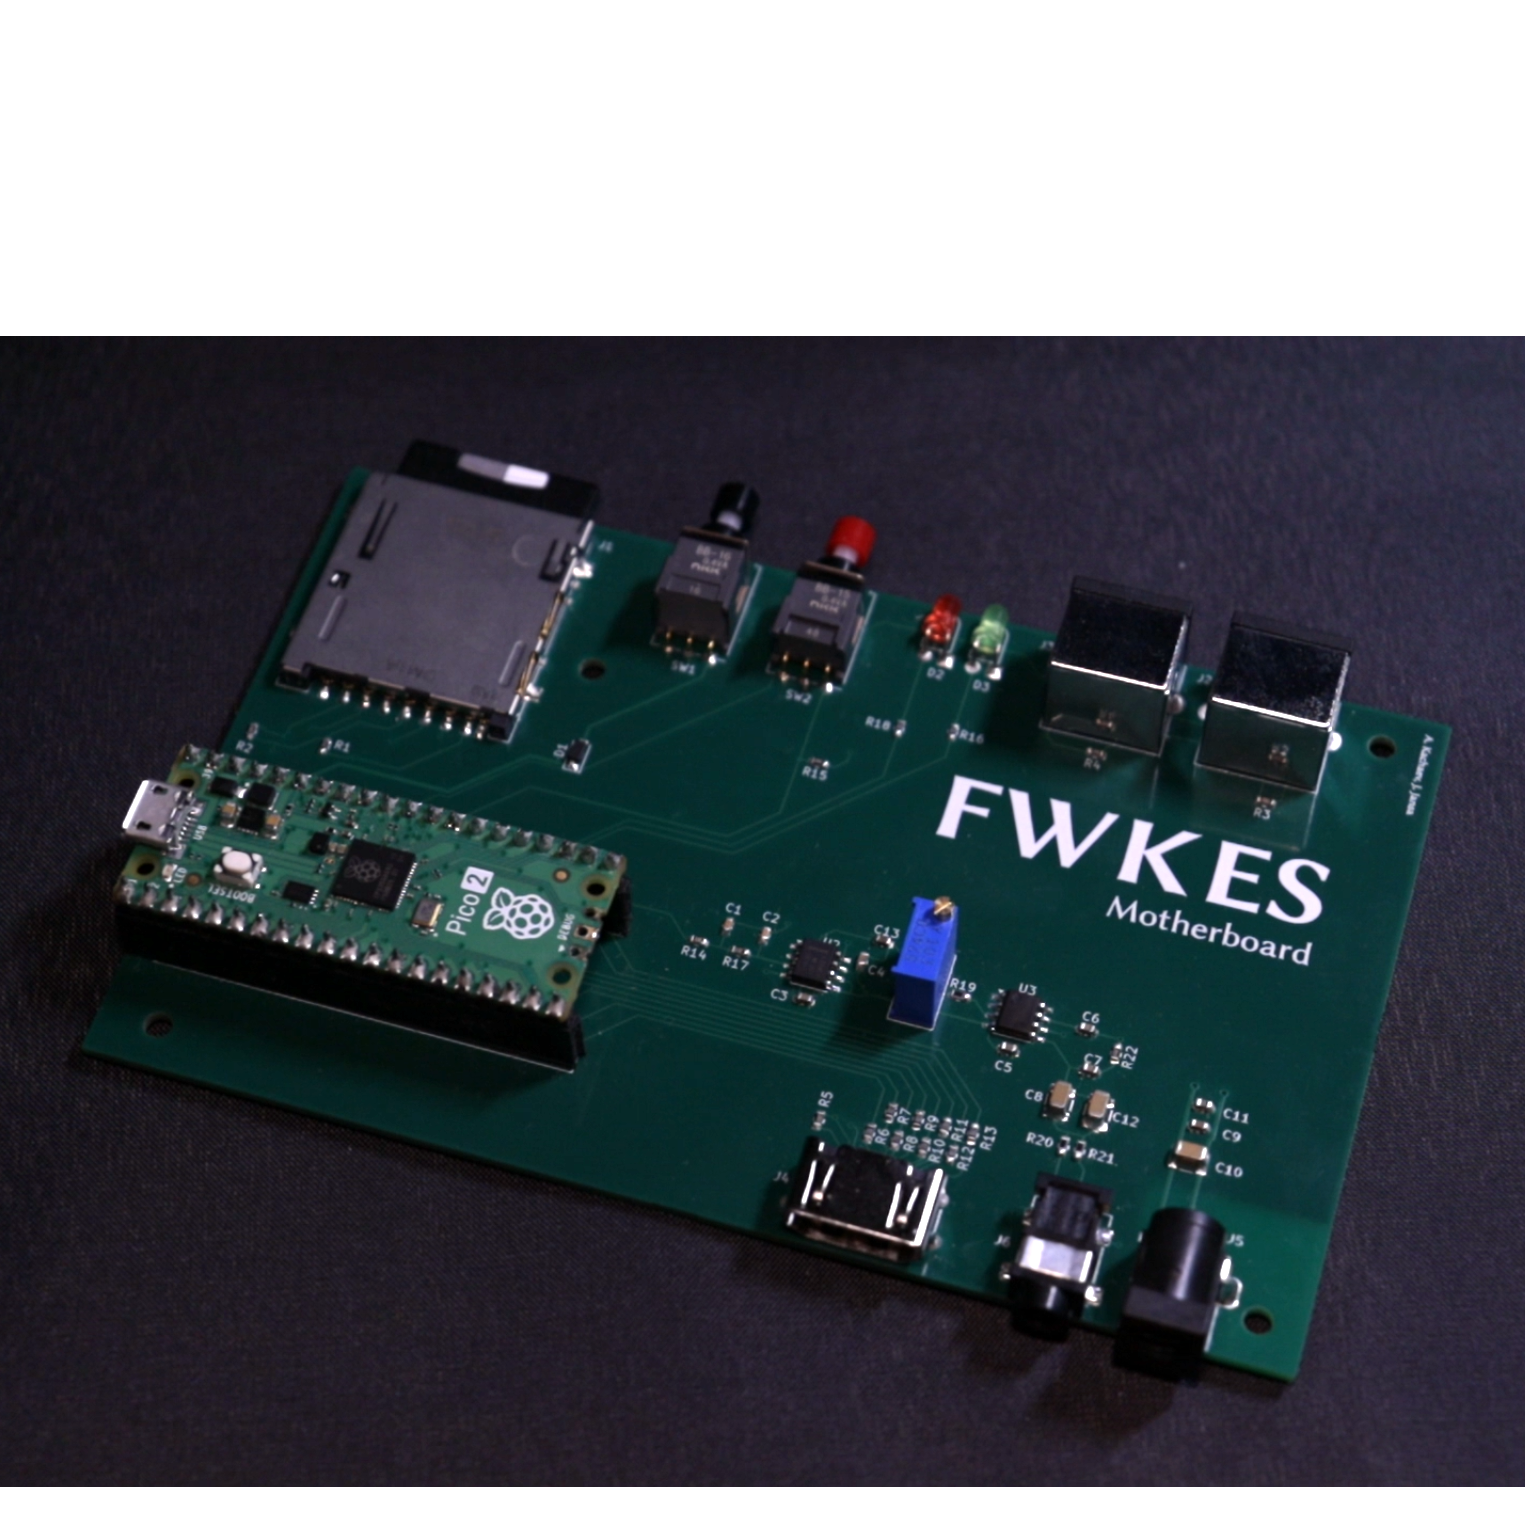
\includegraphics[width=0.75\textwidth]{images/motherboard.png}
    \caption{Vyrobená základní deska.}
    \label{fig:motherboard}
\end{figure}

Celý hardware byl navrhován s důrazem na stabilitu, čistotu signálu a dlouhodobou spolehlivost.
Kompletní návrh schématu i desky plošných spojů (DPS) byl vypracován v open-source programu KiCad.
Jedním z problémů bylo integrovat mikrokontrolér spolu s citlivými analogovými (audio) a
vysokofrekvenčními obvody (HDMI a SD karta) na omezeném prostoru. Celé elektrické schéma zapojení
základní desky a návrh DPS je možné najít v přílohách A~a~B.

\section{Napájení}

Celý systém, včetně ovladačů, je napájen od 5 voltů skrz standardní koaxiální napájecí konektor s
průměrem 5.5mm, který používají spotřebitelské adaptéry 5V DC. Díky tomu lze zařízení připojit do
elektrické sítě pomocí standardního adaptéru.

Pro zvětšení stability napájení a zjednodušení návrhu, DPS byla navrhnuta jako 4vrstvová
deska, což znamená, že má 2 signálové vrstvy na přední a zadní stráně, a 2 napájecí
vrstvy uvnitř pro VCC a GND. Díky tomu lze výrazně zkrátit délku napájecích cest a zvýšit stabilitu
napájení a logiky.

\section{Video výstup HDMI}

Ačkoliv mikrokontrolér RP2350 nedisponuje nativním hardwarovým řadičem pro HDMI, emulátor generuje
digitální obrazový signál pomocí softwarově definovaného protokolu na bázi DVI, který je
zpětně-kompatibilní s HDMI, jelikož oba využívají technologii TMDS pro přenos video dat. Video
signal z mikrokontroléru je fyzicky vyveden přes standardní HDMI konektor.

Signálové piny GPIO mikrokontroléru jsou k HDMI konektoru připojeny přes sériové rezistory o hodnotě
220~$\Omega$. Toto řešení vychází z obvodu adaptéru Adafruit DVI Breakout, který jsme zpočátku
používali, a je založen na informaci z oficiální specifikace DVI, sekce \textit{T.M.D.S. Electrical
Specification}.\cite{dvi-spec}

Při integrování na plošný spoj byla věnována pozornost trasování těchto vysokofrekvenčních signálů.
Obrazová data jsou vedena jako diferenciální páry (tři datové a jeden hodinový kanál). Pro zachování
fázové synchronizace barevných složek musely být délky jednotlivých vodičů v páru i párů mezi sebou
striktně vyrovnány. Všechny tyto trasy navíc vedou nepřerušovaně nad vnitřní zemní rovinou, aby byla
dodržena charakteristická diferenciální impedance 100~$\Omega$\cite{dvi-spec}.

\section{Rozhraní SD karty}

Pro ukládání herních ROM souborů a uživatelských dat je na desce integrován slot pro paměťovou
kartu. Z elektrického hlediska je klíčovou součástí tohoto obvodu soustava \textit{pull-up}
rezistorů (typicky 10~k$\Omega$), kterými jsou osazeny linky \textit{CMD} a \textit{DAT0} linky.
Aplikace těchto rezistorů přímo reflektuje požadavky standardu \textit{SD Physical Layer
Specification}.\cite{sd-spec} Během inicializace nebo ve fázích nečinnosti (kdy je sběrnice ve stavu
vysoké impedance) zajišťují tyto rezistory, že signály neplavou (jsou v nedefinovaném stavu), ale
drží stabilní úroveň logické jedničky (3,3~V). Tím se účinně předchází falešným detekcím startu
komunikace vlivem okolního elektromagnetického rušení (EMI). Navíc kryt konektoru SD karty
(shielding) je připojen k zemi, což zajišťuje ochranu proti EMI a elektrostatickému náboji při
vložení SD karty.

\label{sec:dac}
\section{Analogový audio výstup}

Jelikož mikrokontrolér RP2350 nedisponuje integrovaným DA převodníkem, je zvukový signál z
emulovaného APU generován pomocí pulzně šířkové modulace (PWM) na frekvenci 250 kHz. Aby bylo možné
tento digitální signál reprodukovat v běžných audio zařízeních, musí projít procesem rekonstrukce a
zesílení (viz blokové schéma na obrázku \ref{fig:audio_block}).

\begin{figure}[H]
    \centering
    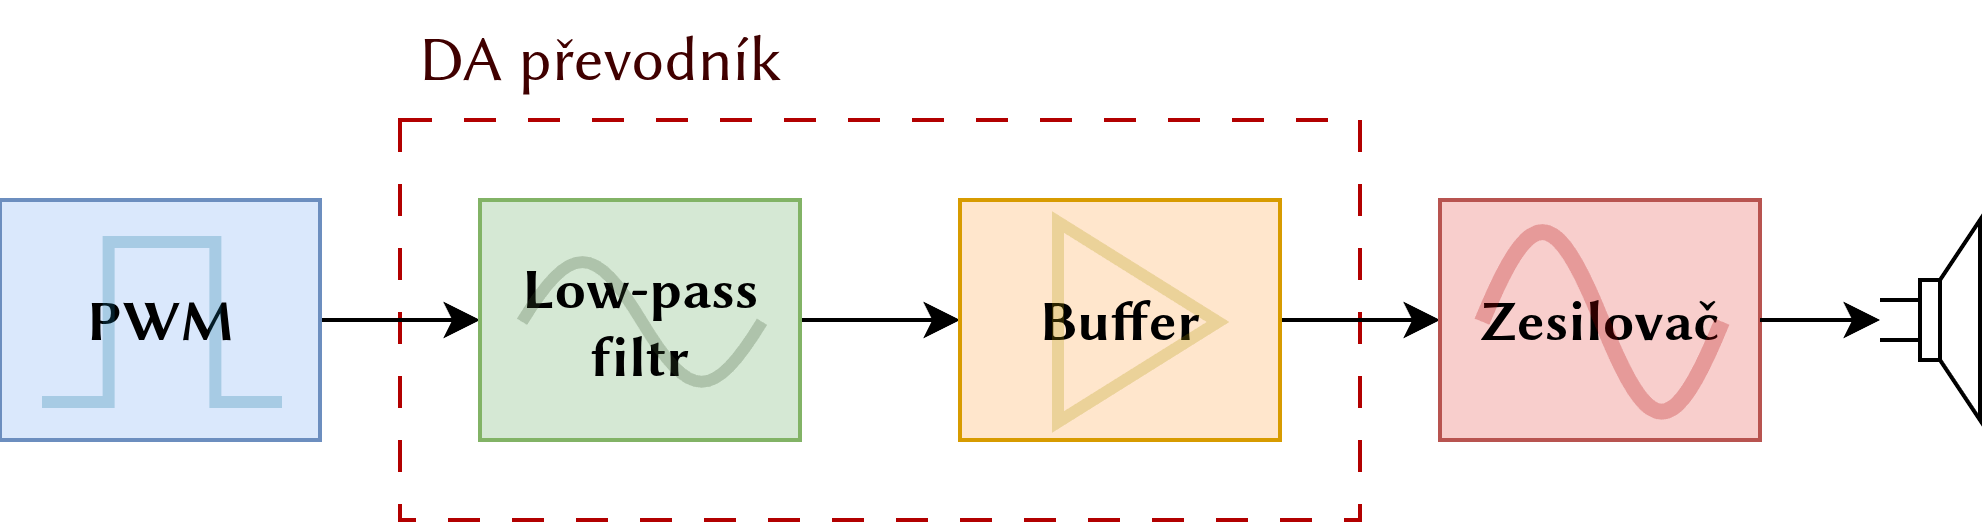
\includegraphics[width=\textwidth]{images/audio_block.png}
    \caption{Blokové schéma analogové částí audio výstupu.}
    \label{fig:audio_block}
\end{figure}

\subsection{Rekonstrukce a předzesílení}

V první fázi je PWM signál veden přes pasivní dolní propust (rekonstrukční filtr). Ten potlačuje
vysokofrekvenční nosnou složku a vyfiltruje užitečnou audio obálku. Následuje aktivní stupeň s
operačním zesilovačem zapojeným jako napěťový sledovač. Tento blok plní dvě úlohy:

\begin{itemize}
    \item Impedanční oddělení -- chrání výstupní piny mikrokontroléru před zátěží a
        stabilizuje signál.
    \item Aktivní filtrace -- zajišťuje strmější odříznutí šumu a zbytků PWM frekvence, čímž
        zvyšuje čistotu zvuku.
\end{itemize}

\subsection{Výkonové zesílení a výstup}

Pro řízení úrovně hlasitosti je v cestě zařazen kalibrační trimr, který slouží jako pasivní dělič
napětí. Finální zesílení signálu na úroveň vhodnou pro sluchátka zajišťuje integrovaný audio
zesilovač LM386. Ten je konfigurován tak, aby poskytoval dostatečnou amplitudu při zachování
stability i při kapacitní zátěži.

Výstupní řetězec je zakončen vazebními kondenzátory, které eliminují stejnosměrnou (DC) složku, a
ochrannými rezistory proti zkratu. Audio výstup je vyveden na standardní \SI{3,5}{\milli\meter} jack
konektor a je dimenzován pro sluchátka s impedancí 32--600,Ω. Podrobný popis jednotlivých
komponentů a kompletní schéma zapojení jsou součástí přílohy E.

% \section{Analogový výstup audio signálu}
%
% % \begin{figure}[htbp]
% %     \centering
% %     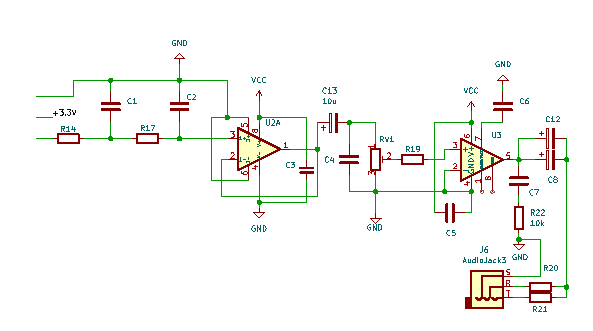
\includegraphics[width=0.85\textwidth]{images/dac.pdf}
% %     \caption{Schéma analogové častí audio výstupu.}
% %     \label{fig:dac}
% % \end{figure}
%
% Tato podkapitola popisuje analogovou část obvodu určenou pro filtraci a~zesílení audio signálu
% generovaného mikrokontrolérem. Návrh vychází z~požadavku na převod
% digitálně reprezentovaného signálu (PWM) na analogový průběh a~jeho následné zesílení na úroveň
% vhodnou pro reprodukci, jak ilustruje schéma na obrázku~\ref{fig:dac}.
%
% \subsection{Vstupní signál a~předzpracování}
%
% Zvukový signál je generován mikrokontrolérem jako výstup emulovaného APU,
% přičemž jednotlivé vzorky jsou reprezentovány digitální hodnotou. Tento signál je následně
% převáděn na výstupní pin mikrokontroléru ve formě \textbf{PWM} (\textit{Pulse Width Modulation}),
% který vzniká změnou střídy (\textit{duty cycle}) digitálního signálu na výstupním pinu, kde šířka pulzu
% odpovídá amplitudě aktuálního audio vzorku. PWM signál obsahuje nízkofrekvenční
% složku (audio) spolu s~vysokofrekvenční nosnou složkou danou frekvencí \SI{250}{\kilo\hertz} (viz
% podkapitola \ref{sub:pwm_configuration}).
%
% Běžná audio zařízení vyžadují spojitý analogový signál, který mikrokontrolér bez interního DA
% převodníku nedokáže přímo generovat. Analogový průběh je proto aproximován v digitální doméně a
% následně rekonstruován pomocí vnějších obvodů.
%
% Za účelem získání analogového signálu je PWM výstup veden přes \textbf{pasivní dolní propust}
% tvořenou rezistory R14, R17 a~kondenzátory C1, C2. Tento filtr realizuje aproximaci integrace PWM
% signálu, čímž dochází k~potlačení vysokofrekvenčních složek a~zachování obálky signálu. Výsledný
% signál je přiveden na neinvertující vstup operačního zesilovače U2A.
%
% \subsection*{První zesilovací stupeň}
%
% Operační zesilovač U2A je zapojen jako napěťový sledovač (buffer), který zároveň funguje jako
% \textbf{aktivní dolní propust}. Toto zapojení plní několik klíčových funkcí:
%
% \begin{itemize}
%     \item Oddělení zdroje signálu (mikrokontroléru) od zátěže.
%     \item Snížení výstupní impedance.
%     \item Stabilizace signálu před dalším zpracováním.
% \end{itemize}
%
% Zpětnovazební síť definuje frekvenční charakteristiku tohoto stupně a~omezuje šířku pásma
% zesilovače, čímž dochází k~dodatečné filtraci vysokofrekvenční složky PWM signálu. Tento krok je
% kritický pro snížení šumu a~nežádoucích artefaktů. Na výstupu zesilovače je zařazen vazební
% kondenzátor C13, který odstraňuje stejnosměrnou složku a~umožňuje přenos pouze střídavé části
% signálu.
%
% \subsection*{Řízení hlasitosti}
%
% Za vazebním kondenzátorem následuje trimr RV1, který slouží jako pasivní dělič napětí
% pro řízení amplitudy signálu (hlasitosti). Trimr je využit pro kalibraci úrovně signálu
% a~není určen k~uživatelskému ovládání.
%
% \subsection*{Druhý zesilovací stupeň}
%
% Operační zesilovač U3 představuje hlavní výkonový stupeň analogové části (audio zesilovač LM386). Je
% zapojen jako neinvertující zesilovač, přičemž jeho zesílení je určeno zpětnovazební sítí
% tvořenou komponenty R22, C5 a~C7. Tato konfigurace umožňuje:
%
% \begin{itemize}
%     \item Dosažení vyšší amplitudy výstupního signálu.
%     \item Částečnou kompenzaci frekvenční charakteristiky.
%     \item Stabilizaci zesilovače při kapacitní zátěži.
% \end{itemize}
%
% Kondenzátor C6 slouží jako \textbf{blokovací (decoupling) kondenzátor} napájení a~potlačuje
% rušení přicházející z~napájecí větve.
%
% \subsection{Výstupní vazba a~připojení zátěže}
%
% Výstupní signál je veden přes paralelně zapojené vazební kondenzátory C12 a~C8. Toto uspořádání
% (typicky kombinace většího elektrolytického a~menšího keramického kondenzátoru) zajišťuje odstranění
% DC složky a~přenos nízkých frekvencí, a~zároveň slouží k~efektivní filtraci vysokofrekvenčního
% rušení díky nízkému ekvivalentnímu sériovému odporu (ESR) keramické varianty. Společně tak bezpečně
% chrání připojené zařízení (např. sluchátka nebo externí zesilovač).
%
% Audio výstup je realizován pomocí konektoru J6 (audio jack), kde výstupní kanál je veden
% přes rezistory R20 a~R21. Tyto rezistory slouží jako:
%
% \begin{itemize}
%     \item ochrana proti zkratu,
%     \item omezení výstupního proudu,
%     \item přizpůsobení impedance.
% \end{itemize}
%
% Výsledný analogový výstup je tak vhodný pro přímé připojení sluchátek (32–600 \si{\ohm}) i
% externích zesilovačů a splňuje požadavky na frekvenční rozsah 20 Hz – 20 kHz při dostatečné
% dynamice.

\section{Mikrokontrolér}

Pro snadnou výměnu mikrokontroléru (respektive vývojové desky Raspberry Pi Pico 2) a zároveň
jednodušší návrh, plošný spoj je vybaven hnízdem, kam se vkládá vývojová deska. Přímá integrace
mikrokontroléru RP2350 a okolního obvodu by ztížilo celkový návrh, zvýšilo by cenu výroby a zároveň
by neumožnilo používat neoficiální vývojové desky (které mohou např. rozšiřovat RAM paměť). Navíc
overclocking zkracuje životnost mikrokontroléru, proto uživatel bude moci vyměnit mikrokontrolér v
případě poruchy.

Tento přístup také umožňuje použití jiných desek založených na mikrokontroléru RP2350. Tak například
je možné použit desku Pimoroni Pico Plus 2, která nabízí 8 MB SRAM a 16 MB Flash pamětí navíc, a
také USB-C konektor.
